\PassOptionsToPackage{unicode=true}{hyperref} % options for packages loaded elsewhere
\PassOptionsToPackage{hyphens}{url}
%
\documentclass[]{article}
\usepackage{lmodern}
\usepackage{amssymb,amsmath}
\usepackage{ifxetex,ifluatex}
\usepackage{fixltx2e} % provides \textsubscript
\ifnum 0\ifxetex 1\fi\ifluatex 1\fi=0 % if pdftex
  \usepackage[T1]{fontenc}
  \usepackage[utf8]{inputenc}
  \usepackage{textcomp} % provides euro and other symbols
\else % if luatex or xelatex
  \usepackage{unicode-math}
  \defaultfontfeatures{Ligatures=TeX,Scale=MatchLowercase}
\fi
% use upquote if available, for straight quotes in verbatim environments
\IfFileExists{upquote.sty}{\usepackage{upquote}}{}
% use microtype if available
\IfFileExists{microtype.sty}{%
\usepackage[]{microtype}
\UseMicrotypeSet[protrusion]{basicmath} % disable protrusion for tt fonts
}{}
\IfFileExists{parskip.sty}{%
\usepackage{parskip}
}{% else
\setlength{\parindent}{0pt}
\setlength{\parskip}{6pt plus 2pt minus 1pt}
}
\usepackage{hyperref}
\hypersetup{
            pdftitle={Systematic review and climate change analysis in Los Lagos Region},
            pdfauthor={Derek Corcoran},
            pdfborder={0 0 0},
            breaklinks=true}
\urlstyle{same}  % don't use monospace font for urls
\usepackage[margin=1in]{geometry}
\usepackage{longtable,booktabs}
% Fix footnotes in tables (requires footnote package)
\IfFileExists{footnote.sty}{\usepackage{footnote}\makesavenoteenv{longtable}}{}
\usepackage{graphicx,grffile}
\makeatletter
\def\maxwidth{\ifdim\Gin@nat@width>\linewidth\linewidth\else\Gin@nat@width\fi}
\def\maxheight{\ifdim\Gin@nat@height>\textheight\textheight\else\Gin@nat@height\fi}
\makeatother
% Scale images if necessary, so that they will not overflow the page
% margins by default, and it is still possible to overwrite the defaults
% using explicit options in \includegraphics[width, height, ...]{}
\setkeys{Gin}{width=\maxwidth,height=\maxheight,keepaspectratio}
\setlength{\emergencystretch}{3em}  % prevent overfull lines
\providecommand{\tightlist}{%
  \setlength{\itemsep}{0pt}\setlength{\parskip}{0pt}}
\setcounter{secnumdepth}{5}
% Redefines (sub)paragraphs to behave more like sections
\ifx\paragraph\undefined\else
\let\oldparagraph\paragraph
\renewcommand{\paragraph}[1]{\oldparagraph{#1}\mbox{}}
\fi
\ifx\subparagraph\undefined\else
\let\oldsubparagraph\subparagraph
\renewcommand{\subparagraph}[1]{\oldsubparagraph{#1}\mbox{}}
\fi

% set default figure placement to htbp
\makeatletter
\def\fps@figure{htbp}
\makeatother

\usepackage[round]{natbib}
\usepackage{booktabs}
\usepackage{longtable}
\usepackage{array}
\usepackage{multirow}
\usepackage{wrapfig}
\usepackage{float}
\usepackage{colortbl}
\usepackage{pdflscape}
\usepackage{tabu}
\usepackage{threeparttable}
\usepackage{threeparttablex}
\usepackage[normalem]{ulem}
\usepackage{makecell}
\usepackage{xcolor}
\usepackage[]{natbib}
\bibliographystyle{plainnat}

\title{Systematic review and climate change analysis in Los Lagos Region}
\author{Derek Corcoran}
\date{2020-11-29}

\begin{document}
\maketitle

\hypertarget{systematic-review}{%
\section{Systematic review}\label{systematic-review}}

\hypertarget{introduction}{%
\subsection{Introduction}\label{introduction}}

One of the strategic targets of the Convention of Biological Conservation is ``By 2020, at least 17\% of terrestrial and inland water, and 10\% of coastal and marine areas, especially areas of particular importance for biodiversity and ecosystem services, are conserved through effectively and equitably managed, ecologically representative and well connected systems of protected areas\ldots{}''
This emphasizes not only that protected areas (PA) are one of the most effective elements to prevent extinctions hence conserve biological diversity, also future of biological and landscape conservation need planned increment in the number of PA and effectiveness in terms of strategic allocation of management and economic efforts \citep{le2013protected, watson2014performance}.
This is why the last decades aspects such as economic limitations and the impact on local stakeholders are been taking into account in order to declare news PA and not only its selection based in ecological knowledge \citep{borrini2004indigenous}.

South America has one of the highest proportions of pa area in the world (15.9\%, \citet{ProtectedAreas}).
In Chile, there are 211 PA in its extension. From those, 187 have national jurisdiction and only 24 international.
In southern Chile, Los Lagos Region is named given this region has the largest proportion of lake's area in the country, with 52 lakes over 3 Km2, and a total area of 2,850 Km2. It has a population of 828,708 \citep{Censo2017} and an extension of 48,583.60 Km2.
This region bases its economy in activities related to primary sectors: livestock, aquaculture and forestry industry \citep{BNC_LosLagos}. Even more, Los Lagos Region presents one of the biggest growth in fisheries and aquaculture growth in comparison with the rest of the country during the last 30 years \citep{Soto-alvaradoDesarrollo}.

According to \citet{ProtectedAreas}, Los Lagos Region has 21 PA in 15,777 Km2 of surface.
An even when includes a large part of the territory, there has been a disconnection with local communities.
This could be because from those 21 PA in the Region, 9 correspond to National Parks (NP) and Natural Monuments (NM) which are IUCN categories that reinforce strict conservation \citep{dudley2008guidelines}.
In addition to that, remoteness of PA can generate disconnection. Given most of the PA are located in remote places, people from developed urban centers do not have, in most of the cases, nexus with PA and their territory \citep{joppa2009high}
Another factor could be a social phenomena, where cultural changes as a product of economic activities such as salmon farming, where the dependency of international markets predominates, transform people in this region do not share a common notion of territory or a regional common agenda (Montecinos, 2009, p.~24)

Among the PA in Los Lagos Region, there are three Andean National Parks: Puyehue National Park (PNP), Vicente Perez Rozales National Park (VPRNP), and Alerce Andino National Park (AANP). PNP, VPRNP, and AANP as all national PA in Chile are under the supervision and administration of the National Forestry Corporation (CONAF). They count with management plans (2008, 2015, and 1997, respectively), which provides a very careful compilation of data. However, these documents have not been correctly updated and they have a lack of information with the changes that have occurred in the last years. For example, between 1995 and 2016 native forests in this area have suffer important losses because of land use changes (mostly land modification to grassland and shrubs, and substitution).
Hence, the area presents an increment of vulnerability in front of climate change \citep{marquet2019biodiversidad}.

Considering relations of PA and local communities, and the importance of the expansion of ecological knowledge to areas that resume the complexity of each PA in order to face specific perturbations or global problematic as climate change in the future, should be a fundamental step in Chile to assure a correct management and projection of PA to the future.
This review revise the ecological literature carry out in these three protected areas and its surroundings in Los Lagos Region in order to generate a base line that allow to project scenarios of climate change to systematic conservation planning in PA.
We made a systematic review of research searching by the names of the three PA: PNP, VPRNP, and AANP; and by the geographical area of Southern Chile.
Doing so, we were able to identified tendencies and gaps in research developed in these three National Parks. We could defined a vision on where to focus new studies that allow systematic conservation plans that includes information to deal with climate change and ensure the biological diversity in Southern Chile.

\hypertarget{methodology}{%
\subsection{Methodology}\label{methodology}}

In order to identify research developed in the focus area, a systematic review of literature was performed through the Web of Knowledge database. Information was categorized according to research areas presented in this project.
Two eligibility criteria were performed: 1. including the name of the National Parks of interest, using keywords at topic level: ``Puyehue National Park'' or ``Vicente Perez Rozales National Park'' or ``Alerce Andino National Park'', and 2. Geographic areas surrounding the National Parks, using keywords at topic level: ``South Central Chile'' or ``North Chilean Patagonia'' or ``Los Lagos Region''. The period of the search included from 1975 until October 2020. Grey-literature was not incorporated in the selection.

Articles selected were categorized by publication year, source title, keywords used, and categories created for the purpose of this review: key component, study location, methodology used, process involved, and study object.
Key components categorized articles according to area of study. This classification included Archaeology \& Paleoecology, Climate \& environment (including studies in climate, environmental conditions, and seismology), Ecosystem functioning \& services, Freshwater biodiversity, Hydrology, Social-ecology, and Species \& distribution (including biogeography, species description, and exotic species).

Study location encompassed categories such as the three National Parks of interest: AANP, PNP, and VPRNP; adjacent areas to NP: Adjacent to AANP, Adjacent to PNP, Adjacent to VPRNP; similar ecosystems to NP: Andes of Los Rios Region, Argentinian Andes, and Neuquen in Argentina; Larger areas that comprise NP: Los Lagos Region, 2 regions, 3 regions, 4 regions, 5 regions, More than 5 regions; Global studies: Chile, Chile \& Argentina; and Close urban centers: Valdivia.

Methodology classified articles based in how data was collected and/or analysed.
Methods included data from the field: field survey, field collection (similar a survey but with samples that need further processes to be analysed, such as dendrochronology or electric fishing), field experiment (that requires modification to one or more conditions in a location, such as transplant or seedling experiments).
Other classifications were modeling (including data analysis such as simulations, correlational and multivariate models, and spatial models), molecular analysis (reconstruction of mt-DNA, isotopes, and genetic analysis), and reviews of literature.
There is a category of social methods, that include both quantitative (surveys an questionnaires) and qualitative (interviews and discussion articles).
Process category makes reference to the question behind the articles and implies which is the mechanism studied (see the list of of 47 options in Table \ref{tab:tabProcess}).

\begin{table}

\caption{\label{tab:tabProcess}Processes mentioned in studies}
\centering
\begin{tabular}[t]{l}
\toprule
Process\\
\midrule
Behavior\\
Chemical composition\\
Climate\\
Climate change\\
Collective action\\
\addlinespace
Communication\\
Community ensemble\\
Composition\\
Connectivity\\
Conservation\\
\addlinespace
Decomposition\\
Distribution\\
Epidemiological\\
Erosion\\
Eutrophication\\
\addlinespace
Feeding\\
Fire activity\\
Fixation\\
Flow prediction\\
Flowering\\
\addlinespace
Forest characterization\\
Functional variation\\
Genetic variability\\
Genetic variation\\
Growth\\
\addlinespace
Iconography\\
Infiltration\\
Invasion\\
LULC\\
Parasitation\\
\addlinespace
Participation\\
Past climate change\\
Past distribution\\
Phylogeography\\
Political-ecology\\
\addlinespace
Pollution\\
Productivity\\
Rainfall partitioning\\
Regeneration\\
Runoff\\
\addlinespace
Seasonal variability\\
Sedimentation\\
Social vulnerability\\
Succession\\
Survival\\
\addlinespace
Topography\\
Vulnerability\\
\bottomrule
\end{tabular}
\end{table}

Study object classification was prepared based on what is the minimum element studied in each article. This included living organisms such as humans (household combustion, people, and urban areas), animals (communities of birds, crustacean, fishes, and herpetofauna; species of Aegorhinus, craspedacusta, Dromiciops, Liolaemus, wild boar, and woodwasp), plants (aquatic plants, Chusquea, Embothrium, ferns, native vegetation, pollen, Proteaceae, Sarmienta), other organims (such as cyanobacteria, Didymosphenia, lichens, and protozoa), and a particular living category given its abundance of publications is forest communities (with focus in one species Austrocedrus, \emph{F. cupressoides}, and Nothofagus; or in more diverse environments as coihue-Rauli-Tepa, forest, native forest, and evergreen trees).

Study objects also included non-living organisms, focusing in geographic elements (basins, groundwater Storage, lakes, runoff, streams, watershed, and also soil and regional subdivision), physical conditions (fires, precipitation, particulate matter, rock art), and data bases.

In order to centered this review in ecological knowledge carry out in the area of study, we focus our search in Los Lagos region research and Andean studies in surrounded areas. We left out coastal systems within the region, specially research based on Chiloé island because local communities keep a traditional way of life and agricultural systems. This was even proposed as Global Importance Agricultural Heritage System (GIAHS) by the Food and Agricultural Organization \citep{FAO2003Chiloe, FAO2008Chiloe}.

\hypertarget{results}{%
\subsection{Results}\label{results}}

\hypertarget{climate-change-analisis}{%
\section{Climate change analisis}\label{climate-change-analisis}}

\hypertarget{climate-change-in-southern-chile}{%
\subsection{Climate change in southern Chile}\label{climate-change-in-southern-chile}}

In order to evaluate possible scenarios of climate change in the given area, we used a polygon comprising the Los Lagos and Los Ríos regions in Chile, and compared them using GCM compareR \citep{fajardo2020gcm}, considering Mean Anual Temperature and Annual Precipitation. The resulting scaled table of comparisson among futures was then use to select models to be used in the project.

We used the simple structure index (ssi) as implemented by the Vegan package \citep{Oksanen_2019, dolnicar1999tale} to test what number of clusters (Between two and eight), was the best way to represent the 32 Compared GCMs. The best representation was five clusters, from each cluster the GCM closest to the centroid of the cluster was selected. The five selected GCMS were cesm1\_bgc, gfdl\_esm2g, ipsl\_cm5a\_lr, miroc\_esm\_chem and mpi\_esm\_lr and the selected GCMs together with the clusters are shown in figure \ref{fig:SelectedGCMs}.

\begin{figure}
\centering
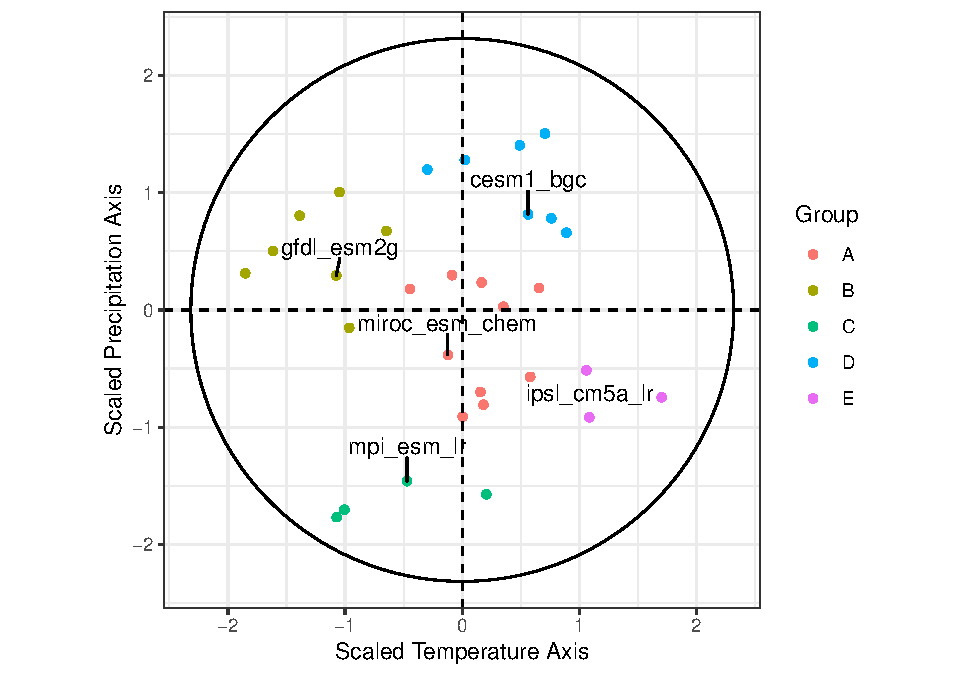
\includegraphics{Review_and_climate_files/figure-latex/SelectedGCMs-1.pdf}
\caption{\label{fig:SelectedGCMs}In this graph we can see the scaled temperature and precipitation axis, the center of the graph represent the ensemble of all models, the five groups represent the clusters selected using kmeans for five groups, the selected GCM of each cluster is shown with a label}
\end{figure}

\hypertarget{present-climate-conditions}{%
\subsubsection{Present climate conditions}\label{present-climate-conditions}}

Once the future GCM models were selected, the 30 seconds resolution maps were downloaded for 2070 and for present conditons from CHELSA \citep{karger2020high}.
The present conditions for the Los Lagos and Los Ríos Region are shown in Figure \ref{fig:PresenteClima}, with a close up to the 10 Km buffer surrounding the park in \ref{fig:PresenteClimaBuffer}. The region is a cold and humid area, with a range in the mean annual temperature from -5.6 to 13 degrees Celsius and a mean of 9.34, and a precipitation range between 858 to 4,537 and a mean of 2,092 mm a year.

\begin{figure}
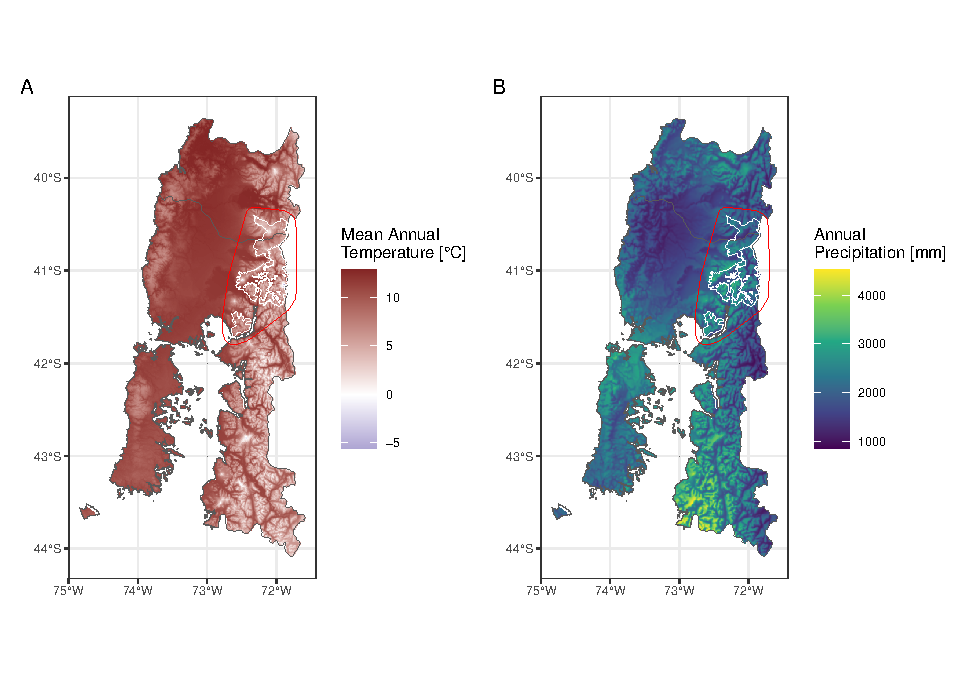
\includegraphics[width=1\linewidth,height=1\textheight]{Review_and_climate_files/figure-latex/PresenteClima-1} \caption{Mean anual temperature in °C (Facet A), and Annual Precipitation mm (Facet B)}\label{fig:PresenteClima}
\end{figure}

The parks concidered in this proyect are in high altitude which leads to even cooler and wetter conditions, with a range from -5.6 to 12.6 and a mean of 8.12 degrees Celsius, and a precipitation range from from 1,176 to 3,410 and a mean of 2,134.51 mm as seen in figure \ref{fig:PresenteClimaBuffer}.

\begin{figure}
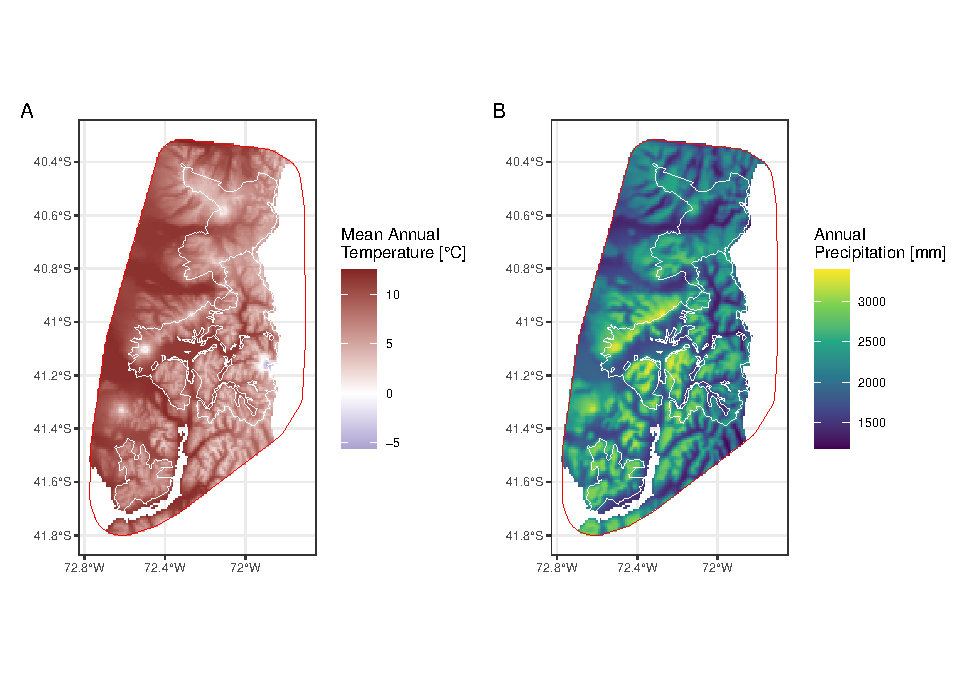
\includegraphics[width=1\linewidth,height=1\textheight]{Review_and_climate_files/figure-latex/PresenteClimaBuffer-1} \caption{Mean anual temperature in °C (Facet A), and Annual Precipitation mm (Facet B) in the three studied national parks white lines, and a 10 km buffer red line}\label{fig:PresenteClimaBuffer}
\end{figure}

\hypertarget{future-scenarios}{%
\subsection{Future scenarios}\label{future-scenarios}}

\hypertarget{future-temperature}{%
\subsubsection{Future temperature}\label{future-temperature}}

\begin{figure}
\centering
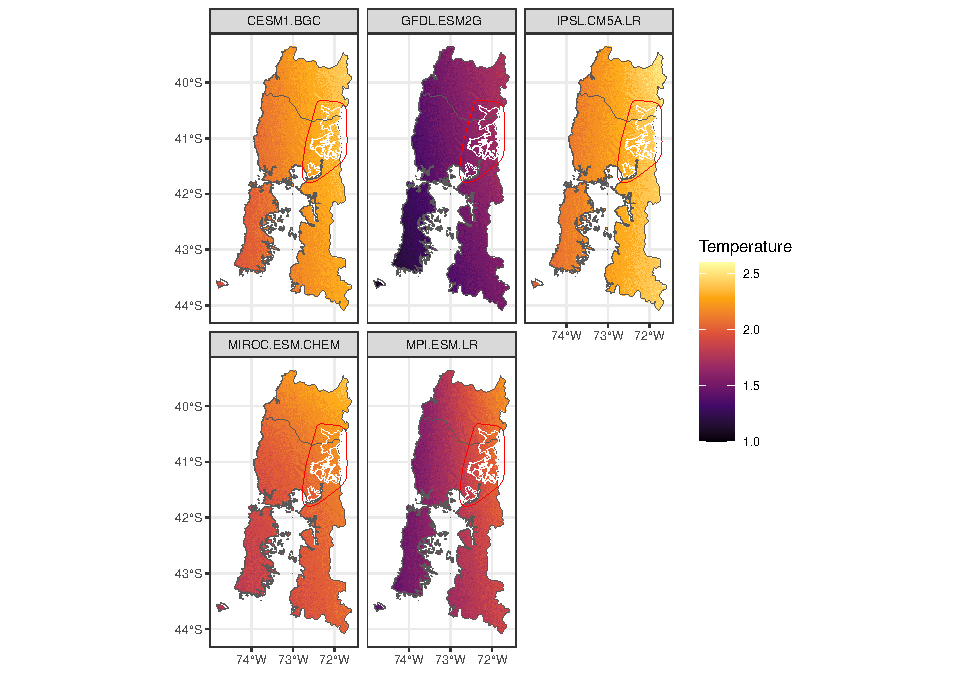
\includegraphics{Review_and_climate_files/figure-latex/DifTemp-1.pdf}
\caption{\label{fig:DifTemp}Changes in future mean annual temperature for the five selected GCMs, the red polygon surrounds the area of influence while the white line demarks the limits of the three protected areas in this proyect}
\end{figure}

As stated above, the four GCMs chosen to explore and model future scenarios are cesm1\_bgc, gfdl\_esm2g, ipsl\_cm5a\_lr, miroc\_esm\_chem and mpi\_esm\_lr. Even when this models include relatively wetter models such as cesm1\_bgc. On average for the whole region, the temperature will rise from 1.5 to 2.28 depending on the GCM (See figure \ref{fig:DifTemp}), but in some areas, it the tempearture rise could be as high as 2.6 degrees Celsius.

As seen in figure \ref{fig:DifTempHull}, those changes are even higher within the parks and it's sorrounding areas, which means the effects of climate change might be even greater.

\begin{figure}
\centering
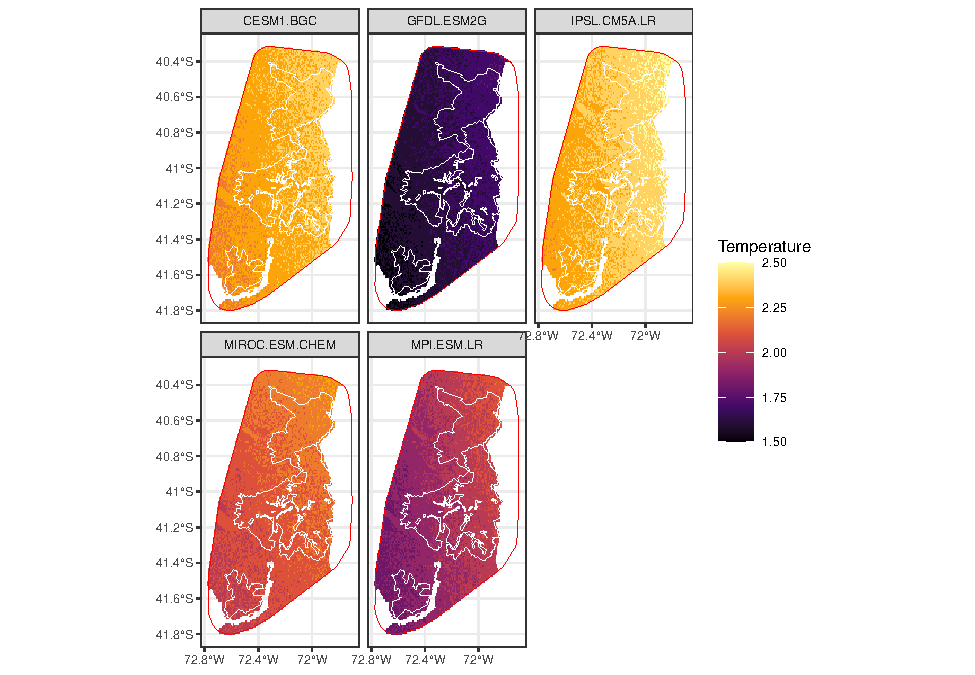
\includegraphics{Review_and_climate_files/figure-latex/DifTempHull-1.pdf}
\caption{\label{fig:DifTempHull}Temperature difference for all five GCMs, for the Close up of the area of influence of the parks}
\end{figure}

\hypertarget{future-precipitation}{%
\subsubsection{Future precipitation}\label{future-precipitation}}

The change in precipitation is predicted to be much more stark, with some areas decreasing in precipitation up to -696 as seen in figure \ref{fig:DifPrec}, this is particularly worrisome, since the ecosystems that are prevalent in the area depend on high precipitation.

\begin{figure}
\centering
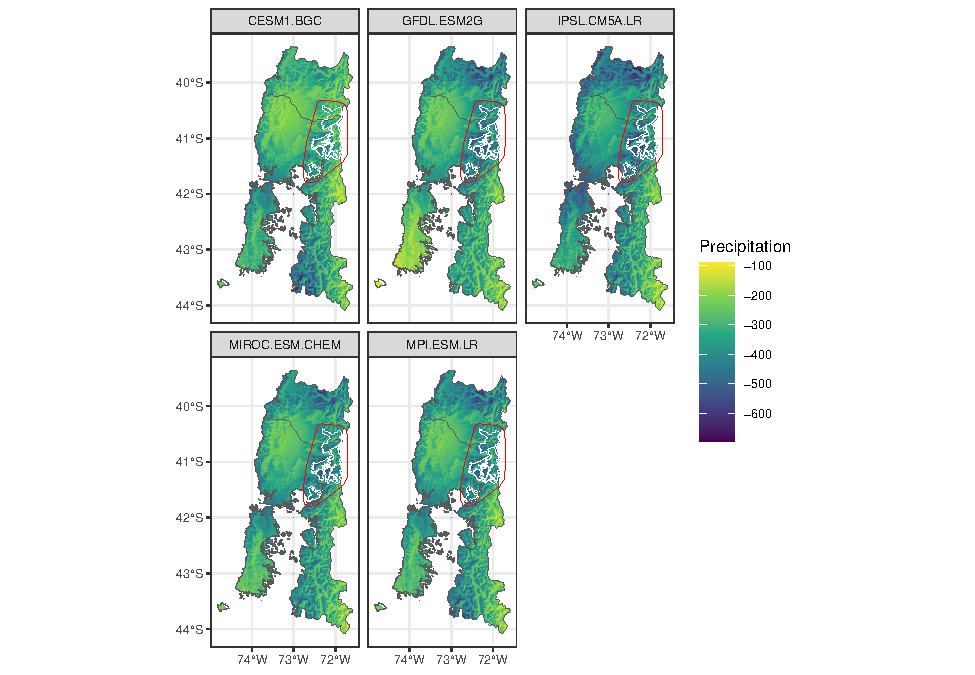
\includegraphics{Review_and_climate_files/figure-latex/DifPrec-1.pdf}
\caption{\label{fig:DifPrec}Changes in precipitation for the different GCMs, the red polygon surrounds the area of influence while the white line demarks the limits of the three protected areas in this proyect}
\end{figure}

\begin{figure}
\centering
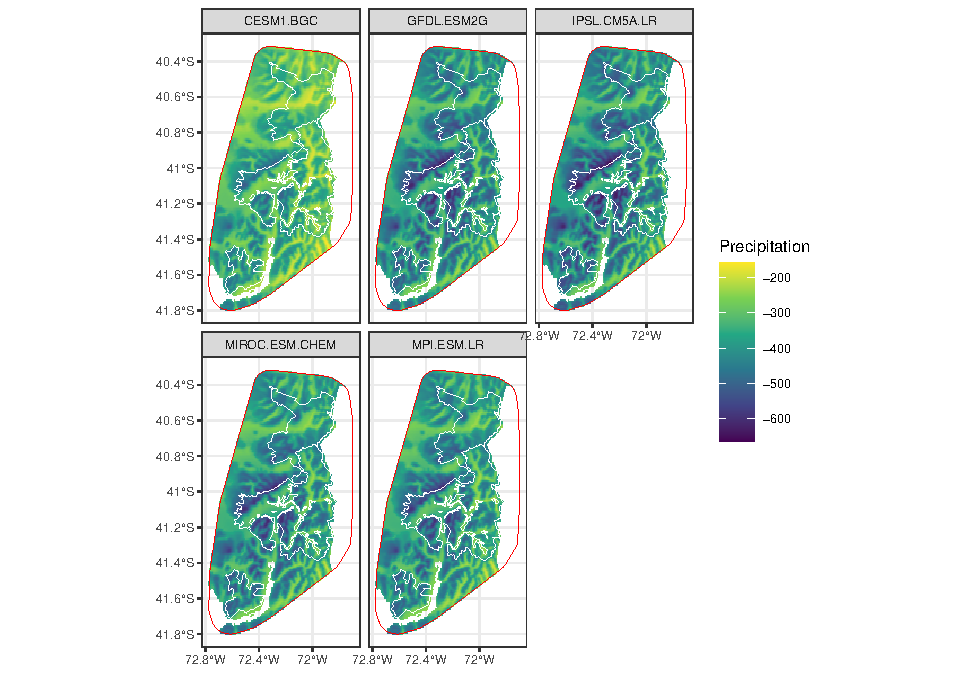
\includegraphics{Review_and_climate_files/figure-latex/DifPrecHull-1.pdf}
\caption{\label{fig:DifPrecHull}Precipitation difference for all five GCMs, for the Close up of the area of influence of the parks}
\end{figure}

The range of changes between GCMs will be from from -376.99 to -313.23 mean annual precipitation for the whole area. Again the areas where there is going to be a higher drop in precipitation are mostly inside of the national parks, as seen in figure \ref{fig:DifPrecHull}, with changes in the mean annual precipitation within the are of -412.29 for the wettest models, and -320.96 for the driest models.

\hypertarget{vegetational-formation}{%
\subsection{Vegetational formation}\label{vegetational-formation}}

We used \citet{luebert2009depuracion} to check current vegetational formations as seen in figure \ref{fig:VegHull}

\begin{figure}
\centering
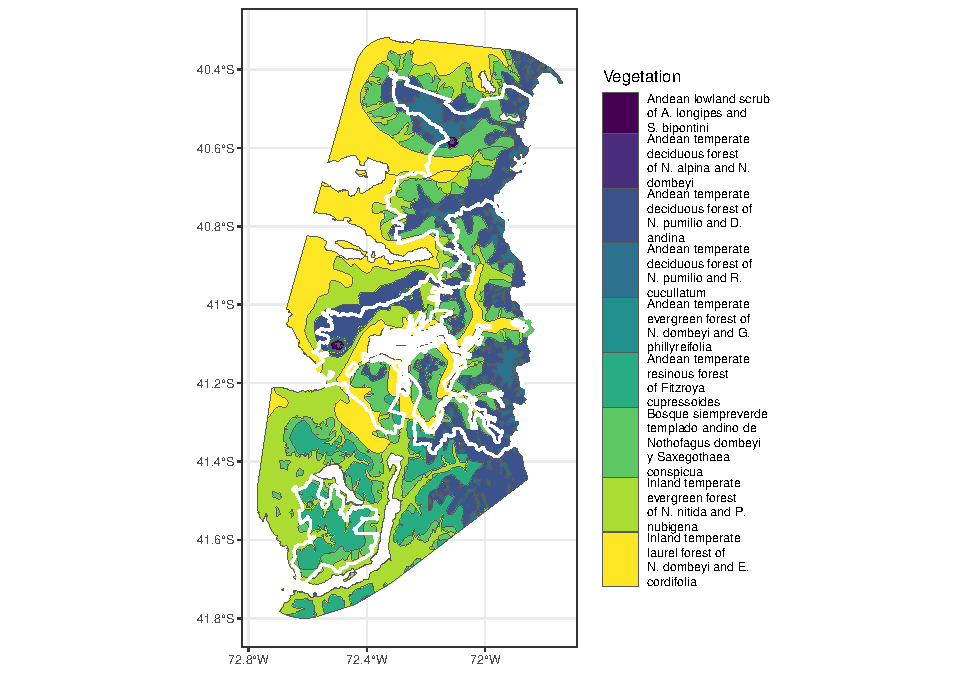
\includegraphics{Review_and_climate_files/figure-latex/VegHull-1.pdf}
\caption{\label{fig:VegHull}Vegetational formation in the influence area of the parks}
\end{figure}

\hypertarget{climatic-analogues}{%
\subsubsection{Climatic analogues}\label{climatic-analogues}}

As seen above, changes in precipitation will be very large. Because of that, we checked which areas in the present have the same climate as it is predicted to be in the future in the national parks and sorrounding areas using the analouges R package \citep{ramirez2011climate}. After doing that, the current vegetational formations of those areas were checked in order to determine possible future vegetation in the area. With that we might better understand the biological consecuences of climate change.

Currently in the National Parks and sorrouding areas, the five most common Vegetational formations are Deciduous forest, Evergreen forest, Laurel forest, Low altitude scrubland and Resinous forest, and in the future, new vegetational formations that would be part of the five most common ones would include Absolute desert, Desert scrub, Sclerophyllous forest and Thorny forest. Of the current five most common formations, the ones that would be reduced as far as that they would either be lost completely or become very rare are Evergreen forest, Low altitude scrubland and Resinous forest

\begin{table}

\caption{\label{tab:TablaForm}Top five vegetation formations for the present and for the different GCMs acording to the analogous climate analysis}
\centering
\fontsize{5}{7}\selectfont
\begin{tabular}[t]{lllllll}
\toprule
Rank & Present & CESM1-BGC & GFDL-ESM2G & IPSL-CM5A-LR & MIROC-ESM-CHEM & MPI-ESM-LR\\
\midrule
1 & Evergreen
forest & Deciduous
forest & Deciduous
forest & Deciduous
forest & Deciduous
forest & Deciduous
forest\\
2 & Deciduous
forest & Sclerophyllous
forest & Sclerophyllous
forest & Sclerophyllous
forest & Sclerophyllous
forest & Sclerophyllous
forest\\
3 & Laurel
forest & Desert
scrub & Thorny
forest & Desert
scrub & Desert
scrub & Desert
scrub\\
4 & Resinous
forest & Thorny
forest & Desert
scrub & Thorny
forest & Thorny
forest & Thorny
forest\\
5 & Low
altitude
scrubland & Laurel
forest & Laurel
forest & Absolute
desert & Laurel
forest & Laurel
forest\\
\bottomrule
\end{tabular}
\end{table}

\hypertarget{land-use}{%
\subsection{Land use}\label{land-use}}

We used \citet{zhao2016detailed} landuse layer, specifically developed for Chile. This is a 30 meter resolution, that

\includegraphics{Review_and_climate_files/figure-latex/unnamed-chunk-6-1.pdf}

\includegraphics{Review_and_climate_files/figure-latex/unnamed-chunk-7-1.pdf}

\begin{table}[H]
\centering
\begin{tabular}{lr}
\toprule
Primary landuse & Percentage\\
\midrule
forests & 59.17\\
grasslands & 12.95\\
Scrub & 10.24\\
Water bodies & 9.34\\
bare land & 6.93\\
\bottomrule
\end{tabular}
\end{table}

\begin{table}[H]
\centering
\begin{tabular}{lr}
\toprule
Secondary landuse & Percentage\\
\midrule
Native Broadleaf renoval & 39.45\\
Native Broad Leaf primary & 18.63\\
Scrub & 10.11\\
Lagos & 8.97\\
grasslands annual & 8.43\\
\addlinespace
Rocks rocky soils & 5.04\\
other Grasslands & 4.40\\
Rocky soil gravels & 1.85\\
\bottomrule
\end{tabular}
\end{table}

\renewcommand\refname{References}
\bibliography{Biblio.bib}

\end{document}
